\chapter{NN potentials}
\label{potentials}
\section{The OPE-Gaussian potential}
\label{OPEG-potential}
The OPE-Gaussian force is a phenomenological NN potential which has been presented by R. Navarro P{\' e}rez, J. E. Amaro, and E. Ruiz Arriola in 2014~\cite{NavarroPerez2014}. In usuall way, this potential can be decomposed to the short-range $V_{\mathrm{short}}(r)$ and the long-range $V_{\mathrm{long}}(r)$ parts,
\begin{equation}
V(r) = V_{\mathrm{short}}(r)\theta(r_{c} - r) + V_{\mathrm{long}}(r)\theta(r - r_{c})\;,
\end{equation}
\label{eq_31}
where $r$ is the internucleon distance and for the OPE-Gaussian potential $r_{c} =$ 3 fm.

The long-range force $V_{\mathrm{long}}(r)$ is, in turn, the sum of the one-pion exchange (OPE) force and the electromagnetic (EM) corrections:
\begin{equation}
V_{\mathrm{long}}(r) = V_{\mathrm{1\pi}} + V_{\mathrm{EM}}\;.
\label{eq_32}
\end{equation}
% the sum of the usual one-pion exchange potential (OPE), $V_{OPE}$, and the electromagnetic corrections for the proton-proton interaction, $V_{em}$.
The OPE potential $V_{\mathrm{1\pi}}$ is the same as the charge-dependent OPE potential used in the PWA93 by the Nijmegen group~\cite{Stoks1993} and the AV18 potential~\cite{Wiringa1995} which reads as
\begin{equation}
V_{\mathrm{\mathrm{1\pi}}}(r) \equiv V_{m, \mathrm{\mathrm{1\pi}}}(r) = \frac{1}{3}mf^{2}\left(\frac{m}{m_{s}}\right)^{2}\left[Y_{m}(r)\vec{\sigma}_{1}\cdot\vec{\sigma}_{2} + T_{m}S_{1,2}\right]\;,
\label{eq_33}
\end{equation}
where $\vec{\sigma}_{1}$ and $\vec{\sigma}_{2}$ denote the Pauli matrices of nucleons 1 and 2, respectively, $S_{1,2}$ is the tensor operator, and $Y_{m}(r)$ and $T_{m}(r)$ are the Yukawa and tensor functions,
\begin{equation}
\begin{split}
S_{12} &= 3\left(\vec{\sigma}_{1}\cdot\hat{r}~\vec{\sigma}_{2}\cdot\hat{r}\right) - \vec{\sigma}_{1}\cdot\vec{\sigma}_{2}\;,~\hat{r} = \frac{\vec{r}_{1} - \vec{r}_{2}}{\left|\vec{r}_{1} - \vec{r}_{2}\right|}\;, \\
Y_{m}(r) &= \frac{e^{-mr}}{mr}\;,\\
T_{m}(r) &= \frac{e^{-mr}}{mr}\left(1 + \frac{3}{mr} + \frac{3}{(mr)^{2}}\right)\;.
\end{split}
\label{eq_34}
\end{equation}
The scalling mass $m_s$ in Eq.~(\ref{eq_33}) is the charged-pion mass $m_{\pi^{\pm}}$, the average value of the pion mass $m = \frac{1}{3}(m_{\pi^{0}} + 2m_{\pi^{\pm}})$ = 138.057 MeV, $f = \sqrt{0.075} \approx 0.274$ is the pion coupling constant, for all pairs of nucleons ($pp$, $np$, $nn$). 
%and depends on a given pair of NN interactions ($pp$, $nn$, $np$) via pion exchange for the corresponding vertex of the Feynman diagram, i.e., $f_{pp\pi^{0}}$, $f_{nn\pi^{0}}$, $f_{np\pi^{-}}$ and $f_{pn\pi^{+}}$. According to PWA93, the Nijmegen group found that these coupling constants differ very little from each other, but due to charge symmetry\footnote{Charge symmetry is an approximate symmetry in which, if not take into account the electromagnetic force, then the interaction in the $nn$, $pp$, and $np$ pairs in the same quantum states are indistinguishable, and this, in turn, one can mean that the nuclear force can be considered as charge independent. Therefore, a proton and a neutron are considered as two states of one particle --- a nucleon.}~($f^{2}_{pp\pi^{0}} = -f_{nn\pi^{0}} f_{pp\pi^{0}}$) they were chosen approximately charge independent, i.e., $f^{2}_{pp\pi^{0}} = -f_{nn\pi^{0}} f_{pp\pi^{0}}= (f_{np\pi^{-}} f_{pn\pi^{+}})/\sqrt{2}\equiv f^{2} = 0.075$. 
As a result, charge dependence is yield only due to the difference between the charged $m_{\pi^{\pm}}$ and neutral $m_{\pi^{0}}$ pion mass and leads to
\begin{equation}
\begin{split}
V^{pp}_{\mathrm{\mathrm{1\pi}}}(r) &= V^{nn}_{\mathrm{1\pi}} \neq V^{np}_{1\pi}\;.\\  
%f^{2}_{p}V_{\mathrm{\mathrm{1\pi}}, m_{\pi^{0}}}(r)\; \\
%V^{np}_{\mathrm{\mathrm{1\pi}}}(r) &= -f^{2}_{0}V_{\mathrm{\mathrm{1\pi}}, m_{\pi^{0}}}(r) + (-1)^{T + 1}2f^{2}_{c}V_{\mathrm{\mathrm{1\pi}}, m_{\pi^{\pm}}}(r)\;,
\end{split}
\label{eq_35}
\end{equation}
%where $T$ is the total isospin of two nucleons and the following definitions
%\begin{equation}
%\begin{split}
%f^{2}_{p} &\equiv f_{pp\pi^{0}}f_{pp\pi^{0}}\;,~f^{2}_{n} \equiv f_{nn\pi^{0}}f_{nn\pi^{0}}\;, f^{2}_{p} = f^{2}_{n}\;,\\
%f^{2}_{0} &\equiv -f_{nn\pi^{0}}f_{pp\pi^{0}},~2f^{2}_{c}\equiv f_{np\pi^{-}}f_{pn\pi^{+}}\;.
%\end{split}
%\label{eq_351}
%\end{equation}
The EM corrections correspond to the $np$ and $pp$ potentials. The $np$ potential contains only a magnetic moment (MM) interaction 
\begin{equation}
V^{np}_{\mathrm{EM}} = V^{np}_{\mathrm{MM}}(r) = -\frac{\alpha\mu_{n}}{2m_{n}r^{3}}\left(\frac{\mu_{p}S_{1,2}}{2m_{p}} + \frac{\vec{L}\cdot\vec{S}}{\mu}\right)\;,
\label{eq_36}
\end{equation}
where $m_{n}$ and $m_{p}$ are the neutron and proton masses, $\mu$ is the reduced mass of the nucleon, $\mu_{n}$ and $\mu_{p}$ are the neutron and proton magnetic moments, $\vec{L}$ and $\vec{S}$ denote the angular momentum and spin operator, respectively, and $\vec{L}\cdot\vec{S}$ is the 2N spin-orbit operator. The $pp$ EM potential contains one- and two-photon exchange, vacuum polarization and a magnetic moment interaction
\begin{equation}
V^{pp}_{\mathrm{EM}} = V^{pp}_{\mathrm{C_{1}}}(r) + V^{pp}_{\mathrm{C_{2}}}(r) + V^{pp}_{\mathrm{VP}}(r) + V^{pp}_{\mathrm{MM}}(r)\;,
\label{eq_37}
\end{equation}
with detalied expressions given in Eqs. (9-12) of Ref.~\cite{Perez2013}
%\begin{equation}
%\begin{split}
%V^{pp}_{\mathrm{C_{1}}}(r) &= \frac{\alpha^{\prime}}{r}\;, \\
%V^{pp}_{\mathrm{C_{2}}}(r) &= \frac{\alpha\alpha^{\prime}}{M_{p}r^{2}}\;,\\
%V_{\mathrm{VP}}(r) &= \frac{2\alpha\alpha^{\prime}}{3\pi r}\int\limits_{1}^{\infty}e^{-2m_{e}rx}\left(1 + \frac{1}{2x^{2}}\right)\frac{\sqrt{x^{2} - 1}}{x^{2}}\mathrm{d}x\;,\\
%V^{pp}_{\mathrm{MM}} &= - \frac{\alpha}{4M^{2}_{p}r^{3}}\left[\mu^{2}_{p}S_{1,2} + 2(4\mu_{p} - 1)\vec{L}\cdot\vec{S}\right]\;.
%\label{eq_38}
%\end{split}
%\end{equation}
%All these potentials Eq.~(\ref{eq_38}) are used for distances $r_{c} \gtrsim$ 3 fm. It was also taken into account the energy dependence, expressed in terms of a parameter
%\begin{equation}
%\alpha^{\prime} = \alpha\frac{1 + \frac{2k^{2}}{M^{2}_{p}}}{\sqrt{1 + \frac{k^{2}}{M^{2}_{p}}}}\;,
%\end{equation}
%where $k$ is the center of mass momentum, $\alpha$ is the fine structure constant.

Below $r_{c}$ = 3 fm the short-range part $V_{short}(r)$ of the OPE-Gaussian force is built from 18 spin-isospin operators $\hat{O}_{n}$, 16 of these operators are the same as in the AV18 model~\cite{stoks1993partial}. Among them 14 operators are charge-independent,
%16 are the same as in the AV18 model, see~\cite{Wiringa1995}, the set of 14 operators are charge-independent, which are denoted as $c, \tau, \sigma, \sigma\tau, t, t\tau, ls, ls\tau, l2$, and are given by
\begin{equation}
\begin{split}
\hat{O}_{i\in\left[1, 14\right]} = &\lbrace\mathds{1}, \vec{\tau}_{1}\cdot\vec{\tau}_{2}, \vec{\sigma}_{1}\cdot\vec{\sigma}_{2}, (\vec{\sigma}_{1}\cdot\vec{\sigma}_{2})(\vec{\tau}_{1}\cdot\vec{\tau}_{2}), S_{12}, S_{12}(\vec{\tau}_{1}\cdot\vec{\tau}_{2}),\\ &\vec{L}\cdot\vec{S}, \vec{L}\cdot\vec{S}(\vec{\tau}_{1}\cdot\vec{\tau}_{2}), \!\vec{L}^{2}, \!\vec{L}^{2}(\vec{\tau}_{1}\cdot\vec{\tau}_{2}), \\ &\!\vec{L}^{2}(\vec{\sigma}_{1}\cdot\vec{\sigma}_{2}), \!\vec{L}^{2}(\vec{\sigma}_{1}\cdot\vec{\sigma}_{2})(\vec{\tau}_{1}\cdot\vec{\tau}_{2}), (\vec{L}\cdot\vec{S})^{2}, (\vec{L}\cdot\vec{S})^{2}(\vec{\tau}_{1}\cdot\vec{\tau}_{2})\rbrace\;.
\end{split}
\label{firspart}
\end{equation}
The remaining operators
\begin{equation}
\begin{split}
\hat{O}_{i\in\left[15, 18\right]} = &\lbrace T_{12}, (\vec{\sigma}_{1}\cdot\vec{\sigma}_{2}),  \!\vec{L}^{2}T_{12}, \!\vec{L}^{2}(\vec{\sigma}_{1}\cdot\vec{\sigma}_{2})T_{12}\rbrace\;,
%O_{i\in\left[15, 21\right]} = &\lbraceT_{12}, (\vec{\sigma}_{1}\cdot\vec{\sigma}_{1}), T_{12}S_{12}T_{12}, (\tau_{z1} + \tau_{z2}),\\&(\vec{\sigma}_{1}\cdot\vec{\sigma}_{2})(\tau_{z1} + \tau_{z2}), L^{2}T_{12}, L^{2}(\vec{\sigma}_{1}\cdot\vec{\sigma}_{2})T_{12}\rbrace\;,
\label{secondpart}
\end{split}
\end{equation}
with $T_{12} = 3\tau_{z1} \tau_{z2} - \vec{\tau}_{1}\cdot\vec{\tau}_{2}$ introduce charge dependence.
Each element of sets (\ref{firspart}-\ref{secondpart}) is multiplied by a sum of four Gaussian functions $F_{i, n}(r) = V_{i,n} exp(-r^{2}/(2a^{2}_{i}))$, where $a_{i} = \frac{a}{1 + i}$ and $V_{i,n}$ are the strength coefficients. Thus
\begin{equation} 
V_{\mathrm{short}}(r) = \sum_{n = 1}^{18}\hat{O}_{n}\left[\sum_{i = 1}^{4}V_{i, n}F_{i, n}(r) \right]\;.
\end{equation}
\begin{table}
\begin{center}
\begin{tabular}{|c|c|c|c|c|}
\hline
Operator &$V_{1, n}$& $V_{2, n}$& $V_{3, n}$ & $V_{4, n}$ 								   \\ \hline
$\mathds{1}$     	 & -19.28330126 & 126.28715008 & -648.61345585 & 694.49367435    \\ \hline
$\vec{\tau}_{1}\cdot\vec{\tau}_{2}$  	 & 2.36233395   &-25.47505195  & 130.03224633  &-284.71844492	   \\ \hline
$\vec{\sigma}_{1}\cdot\vec{\sigma}_{2}$     & 6.05581487   &-75.18832503  & 372.41961972  &-530.80008401    \\ \hline
$\tau\sigma$ & 7.36008330   &-48.55160272  &273.71591816   &-349.00547346    \\ \hline
$(\vec{\sigma}_{1}\cdot\vec{\sigma}_{2})(\vec{\tau}_{1}\cdot\vec{\tau}_{2})$& 1.99828652   &-22.12164190  &70.84584496    &-50.72248959     \\ \hline
$S_{12}, S_{12}(\vec{\tau}_{1}\cdot\vec{\tau}_{2})$& 15.02271531  & -38.34776035 & 183.80564790  & -160.48060286   \\ \hline
$\vec{L}\cdot\vec{S}$& -2.61725312  & 39.43014573  &-217.03270342  &-109.64162556    \\ \hline
$\vec{L}\cdot\vec{S}(\vec{\tau}_{1}\cdot\vec{\tau}_{2})$& 0.01009424   &2.59116238    &-26.57555840   &-77.56809604     \\ \hline
$\!\vec{L}^{2}, \!\vec{L}^{2}(\vec{\tau}_{1}\cdot\vec{\tau}_{2})$& 1.43519736   &-23.58906341  &67.86552330    &144.11773134     \\ \hline
$\!\vec{L}^{2}(\vec{\sigma}_{1}\cdot\vec{\sigma}_{2})$&-0.41138176   &8.33346137    &-82.98819447   & 175.09618737    \\ \hline
$\!\vec{L}^{2}(\vec{\sigma}_{1}\cdot\vec{\sigma}_{2})(\vec{\tau}_{1}\cdot\vec{\tau}_{2})$&-0.09972181   &2.25339230    &-51.87819771   &175.08890636 	   \\ \hline
$(\vec{L}\cdot\vec{S})^{2}$&-0.26615545  &6.63257735    &-55.34306118   &100.71528331 	   \\ \hline
$(\vec{L}\cdot\vec{S})^{2}(\vec{\tau}_{1}\cdot\vec{\tau}_{2})$&0.46072934   &-11.65544792   &150.58275714   &-302.07573779    \\ \hline
$ls2\tau$    &0.71538487   &-18.88652666   &141.73160452   &-182.73368764    \\ \hline
$T_{12}$&0.63788724   &-7.90421846    &24.23180376    &-19.73899169      \\ \hline
$(\vec{\sigma}_{1}\cdot\vec{\sigma}_{2})$   &-0.63788724  &7.90421846     &-24.23180376   &19.73899169       \\ \hline
$ \!\vec{L}^{2}T_{12}$&-0.10631454  &1.31736974     &-4.03863396    &3.28983195        \\ \hline
$ \!\vec{L}^{2}(\vec{\sigma}_{1}\cdot\vec{\sigma}_{2})T_{12}$ &0.10631454   &-1.31736974    &4.03863396     &-3.28983195       \\ \hline
%$r_{c}$      &2.30347728   &				& 				 &					\\ \hline
\end{tabular}
\caption{The central values of operator coefficients $V_{i, n}$ (in MeV) of the OPE-Gaussian potential. The parameter $a$ is 2.30347728 [fm].}
\label{tableOPEG}
\end{center}
\end{table}
It should be noted that in Ref.~\cite{NavarroPerez2014} there are 21 operators, but three of them ($tT$, $\tau_{z}$ and $\sigma\tau_{z}$) are almost equal zero in practical calculations~\cite{NavarroPerez2014},~\cite{privateArriola} and have been skipped in the final version of the OPE-Gaussian potential. The free parameter $a$, which determines the width of the functions $F_ {i, n}(r)$, together with the operator coefficients $V_ {i, n}$ were fixed from the data NN collected in Granada-2013 database~\cite{Perez2013}.
%, see Table~\ref{tableOPEG}. 

The construction of this database was done in the following steps:
\begin{enumerate}
\item The Granada group collected 8124 available $np$- and $pp$-scattering data taken between 1950 and 2013 in the laboratory energy range $E_{\mathrm{lab}}$ up to 350 MeV. They removed data with unknown or unclear statistical and systematic uncertainties.
\item They performed the least-squares fitting procedure to this database and the deuteron binding energy by the coarse-grained potential and delta-shell representation for the short and intermediate part of the NN interaction in terms of partial-wave decomposition at given scattering energy and angle~\cite{Perez2013, NavarroPerez2015}. 
%After the fitting procedure, the $\chi^{2}$ is calculated and minimized with respect to the fitted potential parameters of the $\delta$-shell potential.
%In addition, they normalized data as an additional contribution to the $\chi^{2}$ based on the proposed idea by Gross and Stadler in Ref.~\cite{gross2008covariant}.  
%\item They performed the least-squares fitting procedure for $np$ scattering below pion production threshold by the coarse-grained potential and delta-shell representation ($\delta$-shell potential) for the short and intermediate part of the NN interaction~\cite{perez2013partial, Perez2013, NavarroPerez2015}. After the fitting procedure, the $\chi^{2}$ is calculated and minimized with respect to the fitted potential parameters of the $\delta$-shell potential.
\item Some sets of data were incompatible with each other. To remove them, R. Navarro P{\' e}rez and collaborators applied the 3$\sigma$-criterion introduced by the Nijmegen group in the PWA93. Namely, for the Gaussian statistical data uncertainties $\Delta O^{data}_{i}$, the residuals for observables $O_{i}$, $\left(O^{data}_{i} - O^{theory}_{i}\right)/\Delta O^{data}_{i}$ should be normal-distributed within a  3$\sigma$-confidence level. Unfortunately, this criterion has disadvantages. One of them is that when non-normal outliers data is rejected, it leads to a significantly improved fitting of compatible data (overestimation)~\cite{Perez2013}. Therefore, they applied the improved 3$\sigma$-criterion~\cite{Perez2013} to the complete database based on the idea of 3$\sigma$ self-consistent rejection given by Gross and Stadler~\cite{gross2008covariant} and again refitted of the parameters. As a result, they obtained the new database (the 3$\sigma$ self-consistent Granada-2013 database), that incorporates 6713 $pp$ and $np$ data and confirmed good statistical properties of their $\chi^{2}$ fit with the value of $\chi^{2}$/datum = 1.05.
%~\footnote{It should be noted that the $\chi^{2}$/datum value is given by $\chi^{2}/N_{\mathrm{dof}}$, where $N_{\mathrm{dof}} = N - P$ is the number of degrees of freedom depending on the number of data, $N$, and the number of parameters, $P$. $N = N^{\mathrm{exp}}_{data} + N^{\mathrm{norm}}_{data}$, where $N^{\mathrm{exp}}_{data}$ is the number of data points and $ N^{\mathrm{norm}}_{data}$ the number of estimated normalizations.}.
Having the database and emerging phase-shifts it was possible to fix 42 free partial-wave parameters of the OPE-Gaussian potential which are linear functions of operator coefficients $V_{i, n}$~\cite{NavarroPerez2014}. Final, used also in this thesis, values of $V_{i,n}$ are presented in Table~\ref{tableOPEG}. The resulting $\chi^{2}$/datum for the OPE-Gaussian force amounts 1.06 as fitted to data listed in Ref.~\cite{Perez2013}. The performed extensive statistical analysis of data and careful fitting procedures allowed authors of Ref.~\cite{Perez2014} to provide not only the values of free parameters but also their covariance matrix~\cite{Perez2014}. 
%Using this matrix they sampled from the multivariate normal distribution the free parameters $V_{i, n}$ and $a$, and computed their uncertainty~\cite{Perez2014}.
\end{enumerate}
%We have been equipped by the authors of Ref.~\cite{NavarroPerez2014} with a sample of 50 sets of potential coefficients $\lbrace V_{i, n}\rbrace$ and its the central values with their uncertainties, which a little differ from values in paper~\cite{NavarroPerez2014} in given in Table. 
The knowledge of the covariance matrix of parameters allowed authors of Ref.~\cite{Perez2014} to sample, from the multivariate normal distribution another sets of potentials parameters. They provided us with a sample of 50 sets of parameters $\lbrace V_ {i, n}, a\rbrace$ and its central values. Finally, we would like to note, that the OPE-Gaussian potential has a similar structure to the AV18 force and thus it can be regarded as a remastered version of the standard AV18 model. 

% which can be by the formula
%\begin{equation}
%R_{i} = \frac{O^{exp}_{i}-O^{th}_{i}}{\Delta O^{exp}_{i}}
%\end{equation}

\section{The chiral SMS potential}
\label{chiral_model}
%In Chapter~\ref{introduction}, I outlined that the effective field theory of QCD is $\chi$EFT. which is constructed for systems with a separation of scales based on a power con
Choosing nucleons and pions as only particles in the theory the chiral NN potential can be written as
\begin{equation}
V_{2N} =  V_{\mathrm{cont}} + V_{\mathrm{\pi}}
\label{eg:ch1}
\end{equation}
where $V_{\mathrm{cont}}$ is the contact interaction between nucleons and $V_{\pi}$ represents the pion contributions to the two-nucleon potential. The long-range part of nuclear forces is completely determined
by the chiral symmetry of QCD and experimental information on pion-nucleon ($\pi$N) scattering. Moreover, the pion exchange contributions can be separated by the number of exchanged pions at each chiral order of the chiral expansion, i.e.
\begin{equation}
\begin{split}
&V_{1\pi} = V^{(0)}_{1\pi} + V^{(2)}_{1\pi} + V^{(3)}_{1\pi} + V^{(4)}_{1\pi} + V^{(5)}_{1\pi} + \ldots\;,\\
&V_{2\pi} = V^{(2)}_{1\pi} + V^{(3)}_{1\pi} + V^{(4)}_{1\pi} + V^{(5)}_{1\pi} + \ldots\;.
\end{split}
\label{eg:ch2}
\end{equation}
As an example I show the OPE potential at order $Q^{0}$ (LO) given directly in momentum space reads
\begin{equation}
V^{(0)}_{1\pi}(\vec{q}) = -\left(\frac{g_{A}}{2F_{\pi}}\right)\vec{\tau}_{1}\cdot\vec{\tau}_{2}\frac{\vec{\sigma}_{1}\cdot\vec{q}~\vec{\sigma}_{2}\cdot\vec{q}}{q^{2} + m^{2}_{\pi}}\;.
\end{equation}
Here $\vec{q}$ is the relative momentum transfer of the exchanged pion $\vec{q} = \vec{p}^{~\prime} - \vec{p}$, $\vec{p}$ and $\vec{p}^{~\prime}$ are the initial and final relative momenta of the two nucleons in the c.m.s, $\vec{\tau}_{1}$, $\vec{\tau}_{2}$ denote isospin matrices of nucleons 1 and 2, respectively. $g_{A}$ = 1.29 is the pion-nucleon axial coupling constant and $F_{\pi}$ = 92.4 MeV is the pion decay constant. 

Similarly, the contact interaction between nucleons, which plays a role of the short-range part of the NN force takes the form
\begin{equation}
\begin{split}
&V_{\mathrm{cont}} = V^{(0)}_{\mathrm{cont}} + V^{(2)}_{\mathrm{cont}} + V^{(4)}_{\mathrm{cont}} \ldots\;.
\end{split}
\label{eg:ch3}
\end{equation}
The chiral potential with semilocal regularization in momentum space (the SMS potential) has been derived completely up to the fifth-order (N$^{4}$LO) of the chiral expansion by the Bochum-Bonn group~\cite{Reinert2018}. Comparing the previous chiral forces, the authors fixed the $\pi$N low-energy constants (LECs) using the Roy-Steiner analysis~\cite{hoferichter2015matching}, skipped redundant contact terms in the higher order of the chiral expansion (starting at order $Q^{4}$, i.e. N$^{3}$LO), and, using the Granada-2013 database, determined adjustable parameters of the potential from $np$ and $pp$ scattering data and the deuteron binding energy. They also added the four leading contact terms acting in the N$^{5}$LO ($Q^{6}$ order) F-waves from Ref.~\cite{Entem2017} to their N$^{4}$LO, potential obtaining so-called N$^{4}$LO$^{+}$ interaction.
%as a result, they got updated potential as N$^{4}$LO$^{+}$. 
%For example, the chiral expansion of the NN forces at the leading order is visualized schematically in Figure~\ref{LO}.
%\begin{figure}[h]
%\begin{center}
%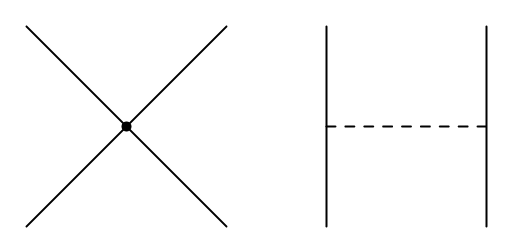
\includegraphics[width=0.5\textwidth]{PhD-text/3_Potentials/LO.png}
%\end{center}
%\caption{The structure of the chiral NN force at the LO order. Solid and dashed lines represent nucleons and pions, respectively.}
%\label{LO}
%\end{figure}
%Implementing local regularization in momentum space~\cite{Reinert2018} the potential $V_{\mathrm{\mathrm{1\pi}}, \Lambda}(m_{\pi})$  
%\begin{equation}
%V_{\mathrm{\mathrm{1\pi}}, \Lambda}(m_{\pi}, \vec{q}) = -\frac{g^{2}_{A}}{4F^{2}_{\pi}}
%\left(\frac{\vec{\sigma}_{1}\cdot\vec{q}~\vec{\sigma}_{2}\cdot\vec{q}}{m^{2}_{\pi} + q^{2}} + C(m_{\pi})~\vec{\sigma}_{1}\cdot\vec{\sigma}_{2}\right)e^{-\frac{m^{2}_{\pi} + q^{2}}{\Lambda^{2}}}\;,
%\end{equation}
%where the constant $C_{\pi}$ depends on the spin-spin part and reads as
%\begin{equation}
%C_{m_{\pi}} = -\frac{\Lambda\left(\Lambda^{2} - 2 m^{2}_{\pi}\right) + 2\sqrt{\pi}m^{3}_{\pi}e^{m^{2}_{\pi}/\Lambda^{2}}\mathrm{erfc}\left(\frac{m_{\pi}}{\Lambda}\right)}{3\Lambda^{3}}\;,
%\end{equation}
%with the error function $\mathrm{erfc}(x)$
%\begin{equation}
%\mathrm{erfc}(x) = \frac{2}{\sqrt{\pi}}\int\limits_{x}^{\infty}e^{-t^{2}}\mathrm{dt}.
%\end{equation}

A general structure of the contact interactions of the chiral SMS force up to fourth-order (N$^{3}$LO) $Q^{4}$ is 
\begin{equation}
\begin{split}
&V^{(0)}_{\mathrm{cont}} = C_{S} + C_{T}\vec{\sigma}_{1}\cdot\vec{\sigma}_{2}\;,\\
&V^{(2)}_{\mathrm{cont}} = C_{1}q^{2} + C_{2}k^{2} + \left(C_{3}q^{2} + C_{4}k^{2}\right)\left(\vec{\sigma}_{1}\cdot\vec{\sigma}_{2}\right) + \frac{i}{2}C_{5}\left(\vec{\sigma}_{1}\cdot\vec{\sigma}_{2}\right)\cdot\left(\vec{k}\times\vec{q}\right)\\
&~~~~~~~~~+ C_{6}\left(\vec{q}\cdot\vec{\sigma}_{1}\right)\left(\vec{q}\cdot\vec{\sigma}_{2}\right) + C_{7}\left(\vec{k}\cdot\vec{\sigma}_{1}\right)\left(\vec{k}\cdot\vec{\sigma}_{2}\right)\;,\\
&V^{(4)}_{\mathrm{cont}} = D_{1}q^{4} + D_{2}k^{4} + D^{3}q^{2}k^{2} + D_{4}\left(\vec{q}\times\vec{k}\right)^{2}\\
&~~~~~~~~~+\left(D_{5}q^{4} + D_{6}k^{4} + D_{7}q^{2}k^{2} + D_{8}\left(\vec{q}\times\vec{k}\right)^{2}\right)\left(\vec{\sigma}_{1}\cdot\vec{\sigma}_{2}\right)\\
&~~~~~~~~~+\frac{i}{2}\left(D_{9}q^{2} + D_{10}k^{2}\right)\left(\vec{\sigma}_{1} + \vec{\sigma}_{2}\right)\cdot\left(\vec{k}\times\vec{q}\right)\\
&~~~~~~~~~+\left(D_{11}q^{2} + D_{12}k^{2}\right)\left(\vec{\sigma}_{1}\cdot\vec{q}\right)\left(\vec{\sigma}_{2}\cdot\vec{q}\right)\\
&~~~~~~~~~+\left(D_{13}q^{2} + D_{14}k^{2}\right)\left(\vec{\sigma}_{1}\cdot\vec{q}\right)\left(\vec{\sigma}_{2}\cdot\vec{q}\right)\\
&~~~~~~~~~+D_{15}\vec{\sigma}_{1}\cdot\left(\vec{q}\times\vec{k}\right)\vec{\sigma}_{2}\cdot\left(\vec{q}\times\vec{k}\right)\;,
\end{split}
\end{equation}
%Short-range interactions have to be tuned to experimental data. 
where $\vec{k} = (\vec{p} + \vec{p}^{~\prime})/2$ and $C_{S}$, $C_{T}$ $C_{1,\ldots, 7}$ and $D_{1,\ldots, 15}$ are the LECs which determine the strength of short-range interaction and should be find from data. 

The usage of nuclear forces derived from $\chi$EFT in few- and many-body problems demand a local regularization for the pion exchange contributions to reduce the amount of finite-cutoff terms and to avoid divergences after substituting, e.g., into the Lippmann-Schwinger equation. In Ref.~\cite{Epelbaum2015}, the Bochum-Bonn group implemented the regularization of the long-range potential in coordinate space, see Eq.~\ref{reg_coord}. Although such regulator allowed to significantly reduce the long-range cutoff terms, but its application turned out to be difficult for the regularization of 3NFs and currents at higher orders of chiral expansion. 
Therefore, the Bochum group introduced a local regularization scheme of long-range forces in momentum space by emplyoing a regularization of static one-pion exchange contribution~\cite{Reinert2018} in the following way
\begin{equation}
f(p^{\prime}, p) \propto \exp\left(-\frac{\left(m^{2}_{\pi} - \!\vec{\,q}^{2}\right)^{2}}{\Lambda^{2}}\right)\;,
\end{equation}
with the cutoff values of $\Lambda = 400, 450, 550$, and 550 MeV. Such approach, as the authors of Ref.~\cite{Reinert2018} argue contributes only to the short-range terms and does not influence the long-range pion exchange potentials.

Implementing local regularization to the long-range potential and multiplying the contact terms with a non-local Gaussian regulator $\mathrm{exp}\left(-\frac{p^{\prime 2} + p^{2}}{\Lambda^{2}}\right)$ in combination with the very detailed fitting procedure of the NN contact LECs leads to a high-quality potential. Specifically, for the chiral SMS potentials of Ref.~\cite{Reinert2018} obtained with the Granada-2013 database~\cite{NavarroPerez2014} the covariance matrices of its free parameters (LECs) at all chiral orders LO-N$^{4}$LO$^{+}$ have been obtained. The number of free parameters (LECs) is 2, 9, 9, 22, 23, 27 at LO, NLO, N$^{2}$LO, N$^{3}$LO, N$^{4}$LO and N$^{4}$LO$^{+}$, respectively. 
Sample visualization of correlations among the various LECs is given in Figure 10 of Ref.~\cite{Reinert2018} for the chiral N$^{4}$LO$^{+}$ SMS potential with $\Lambda$ = 450 MeV. 

Currently, the chiral SMS NN potential is the interaction delivering the best description of NN data. For example, the SMS N$^{4}$LO$^{+}$ with regularization parameter $\Lambda$ = 450~MeV gives $\chi^{2}$/datum = 1.06 ($np$ scattering data) and $\chi^{2}$/datum = 1.00 ($pp$ scattering data), see Table 4 of Ref.~\cite{Reinert2018} up to 300 MeV. In addition, the availability of covariance matrices of LECs for all chiral cutoffs and orders allows us to study, for the first time for a chiral force, the propagation of uncertainties of NN interaction parameters to 3N continuum observables, see Chapter~\ref{application_cov_mat} and Chapter~\ref{error}. 
%~\cite{Reinert2018} the potential $V_{\mathrm{\mathrm{1\pi}}, \Lambda}(m_{\pi})$ 



